

\newcolumntype{L}[1]{>{\raggedright\let\newline\\\arraybackslash\hspace{0pt}}m{#1}}
\newcolumntype{C}[1]{>{\centering\let\newline\\\arraybackslash\hspace{0pt}}m{#1}}
\newcolumntype{R}[1]{>{\raggedleft\let\newline\\\arraybackslash\hspace{0pt}}m{#1}}

\DeclareMathOperator*{\Max}{Maximizar}

\newcommand{\twocols}[3][0.5]{
\begin{columns}
\begin{column}{#1\textwidth}
#2
\end{column}

\begin{column}{#1\textwidth}  
#3
\end{column}

\end{columns}
}


%\newcommand{\twobytwographics}[12]{
%
%\begin{tabular}{|c|c|}
%\includegraphics[scale=#1]{#2} & \includegraphics[scale=#4]{#5} \\
%#3 &  #6\\
%\includegraphics[scale=#7]{#8} & \includegraphics[scale=#10]{#11}\\
%#9 &  #12
%}


\newcommand{\twographics}[4]{
\twocols{\includegraphics[scale=#1]{#2}}{\includegraphics[scale=#3]{#4}}
}


\newcommand{\gesturemodel}[3]{
\centering #1 \vspace{5pt}
  \twocols[0.35]{
    \frame{ \includegraphics[scale=0.75]{features/#2}}
  }{
        \centering
    \frame{\includegraphics[scale=0.75]{features/#3}} 
  }
}




\newenvironment{myframe}{\begin{frame}  \vspace{-5.9pt} }{\end{frame}}

\newenvironment<>{varblock}[2][\textwidth]{
    \begin{center}
      \begin{minipage}{#1}
        \setlength{\textwidth}{#1}
          \begin{actionenv}#3
            \def\insertblocktitle{#2}
            \par
            \usebeamertemplate{block begin}}
  {\par
      \usebeamertemplate{block end}
    \end{actionenv}
  \end{minipage}
\end{center}}



\newcommand{\blockitemize}[2]{
\begin{block}{#1}
\centering
\begin{itemize}
#2
\end{itemize}
\end{block}
}


\def\mytemparray{}

%
\newcommand\abspos[3]{%
    \bgroup
    \def\mytemparray{{ #2 }}
    \pgfmathparse{\mytemparray[0]} \edef\mya{\pgfmathresult}
    \pgfmathparse{\mytemparray[1]} \edef\myb{\pgfmathresult}
    \pgfmathparse{\mytemparray[2]} \edef\myc{\pgfmathresult} %also possible \pgfmathsetmacro
    \begin{tikzpicture}[remember picture, overlay]
            \node[anchor=#1, opacity=\myc] at ( \mya pt, \myb  pt) {#3};
    \end{tikzpicture}%
        %
    %
    \egroup
%
}

%  \rowcolors{1}{gray!15}{gray!15}

\newcommand{\cellcolorgraphictoc}{\cellcolor{blue!40}}

\newcommand{\graphictocresults}{
\begin{tabular}{C{0.5\linewidth}C{0.5\linewidth}}
 
\includegraphics[scale=0.35]{intro/work/hand_db} & 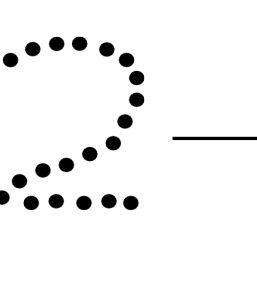
\includegraphics[scale=0.2]{intro/work/representaciones}\\
[-1.5ex] Base de datos de gestos  & Modelo y representaciones de gestos \\
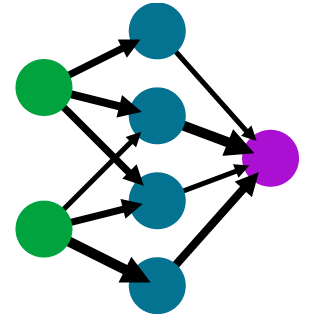
\includegraphics[scale=0.2]{intro/work/cnc} & 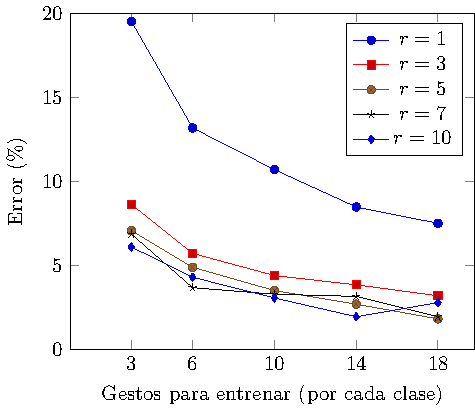
\includegraphics[width=0.34\textwidth]{results/defense_cnc_n} \cellcolorgraphictoc\\  
[-1.5ex] Clasificador Neuronal Competitivo (CNC) & Resultados \cellcolorgraphictoc
\end{tabular}
}

\newcommand{\graphictocdb}{
\begin{tabular}{C{0.5\linewidth}C{0.5\linewidth}}
\cellcolorgraphictoc 

 
\includegraphics[scale=0.35]{intro/work/hand_db} \cellcolorgraphictoc & 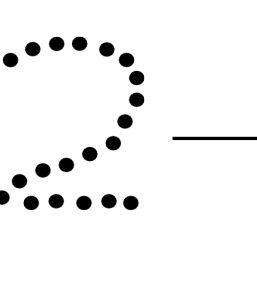
\includegraphics[scale=0.2]{intro/work/representaciones} \cellcolorgraphictoc\\
[-1.5ex] Base de datos de gestos \cellcolorgraphictoc & Modelo y representaciones de gestos \cellcolorgraphictoc \\
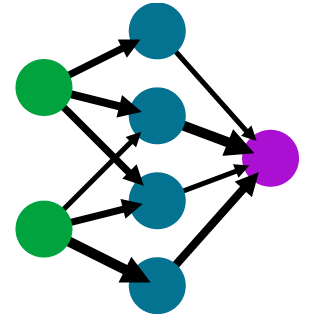
\includegraphics[scale=0.2]{intro/work/cnc} & 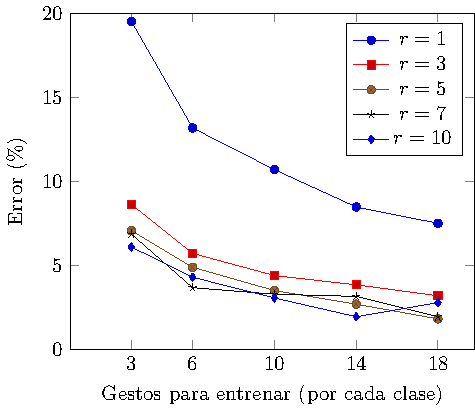
\includegraphics[width=0.34\textwidth]{results/defense_cnc_n} \\  
[-1.5ex] Clasificador Neuronal Competitivo (CNC) & Resultados
\end{tabular}
}

\newcommand{\graphictoccnc}{
  \begin{tabular}{C{0.5\linewidth}C{0.5\linewidth}}
 
\includegraphics[scale=0.35]{intro/work/hand_db} & 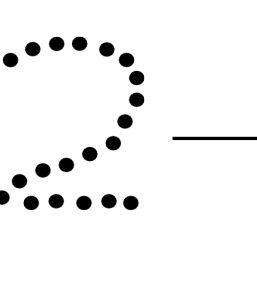
\includegraphics[scale=0.2]{intro/work/representaciones}\\
  [-1.5ex] Base de datos de gestos  & Modelo y representaciones de gestos \\
  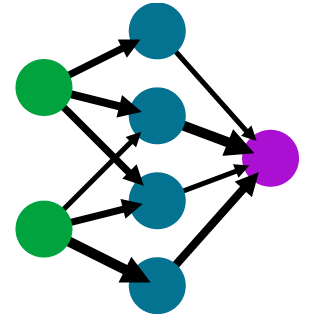
\includegraphics[scale=0.2]{intro/work/cnc} \cellcolorgraphictoc & 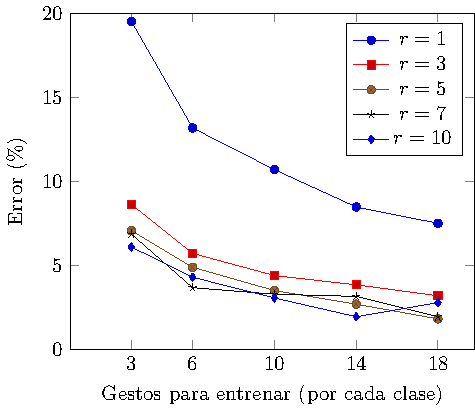
\includegraphics[width=0.34\textwidth]{results/defense_cnc_n} \\  
  [-1.5ex] Clasificador Neuronal Competitivo (CNC) \cellcolorgraphictoc & Resultados
  \end{tabular}
}


\newcommand{\xv}{\ve{x}}
\newcommand{\wv}{\ve{w}}
\newcommand{\cc}{$\ve{cc}$}
\newcommand{\ve}[1]{\mathbf{#1} }
\newcommand{\derivative}[2]{\dv{#1}{#2}}
\newcommand{\dv}[2]{\frac{\partial #1}{\partial #2}}
